\documentclass{tudelft-report}

%% Set up the bibliography
\usepackage{biblatex}
\addbibresource{report.bib}

%% Additional packages and commands
\setlist{itemsep=-2pt} % Reducing white space in lists slightly
\renewcommand{\deg}{\si{\degree}\xspace} % Use \deg easily, everywhere

%% ----------------------------------------------------------------------
%%    Begin of document + Frontmatter (Roman page numbering)
%% ----------------------------------------------------------------------

\begin{document}

\frontmatter

%% Define the main parameters
\title{机器学习算法}
\subtitle{感知机}
\author{我真的不懂忧郁}

\subject{} % Cover only
\affiliation{Delft University of Technology} % Cover only
\coverimage{figures/cover.jpg} % Aspect ratio of 2:3 (portrait) recommended
\definecolor{title}{HTML}{4884d6} % Color for cover title

\makecover

%\begin{titlepage}

\begin{center}

%% Print the title
{\makeatletter
\largetitlestyle\fontsize{45}{45}\selectfont\@title
\makeatother}

%% Print the subtitle
{\makeatletter
\ifdefvoid{\@subtitle}{}{\bigskip\titlestyle\fontsize{20}{20}\selectfont\@subtitle}
\makeatother}

\bigskip
\bigskip

by

\bigskip
\bigskip

%% Print the name of the author
{\makeatletter
\largetitlestyle\fontsize{25}{25}\selectfont\@author
\makeatother}

\bigskip
\bigskip

%% Print table with names and student numbers
\setlength\extrarowheight{2pt}
\begin{tabular}{lc}
    Student Name & Student Number \\\midrule
    First Surname & 1234567 \\
\end{tabular}

\vfill

%% Print some more information at the bottom
\begin{tabular}{ll}
    Instructor: & I. Surname \\
    Teaching Assistant: & I. Surname \\
    Project Duration: & Month, Year - Month, Year \\
    Faculty: & Faculty of Aerospace Engineering, Delft
\end{tabular}

\bigskip
\bigskip

%% Add a source and description for the cover and optional attribution for the template
\begin{tabular}{p{15mm}p{10cm}}
    Cover: & Canadarm 2 Robotic Arm Grapples SpaceX Dragon by NASA under CC BY-NC 2.0 (Modified) \\
    % Feel free to remove the following attribution, it is not required - still appreciated :-)
    Style: & TU Delft Report Style, with modifications by Daan Zwaneveld
\end{tabular}

\end{center}

%% Insert the TU Delft logo at the bottom of the page
\begin{tikzpicture}[remember picture, overlay]
    \node[above=10mm] at (current page.south) {%
        
\includegraphics{figures/logo-black}
    };
\end{tikzpicture}

\end{titlepage}

%\chapter*{Preface}
\addcontentsline{toc}{chapter}{Preface}

\emph{A preface...}

\begin{flushright}
{\makeatletter\itshape
    \@author \\
    Delft, \monthname{} \the\year{}
\makeatother}
\end{flushright}









%\chapter*{Summary}
\addcontentsline{toc}{chapter}{Summary}

\emph{A summary...}


\tableofcontents
%\listoffigures
%\listoftables

\chapter*{Nomenclature}
\addcontentsline{toc}{chapter}{Nomenclature}

\emph{If a nomenclature is required, a simple template can be found below for convenience. Feel free to use, adapt or completely remove.}

\section*{Abbreviations}

\begin{longtable}{p{2.5cm}p{8cm}}
    \toprule
    Abbreviation & Definition \\
    \midrule\endhead % Add abbreviations alphabetically here:
    ISA & International Standard Atmosphere \\
    ... \\
    \bottomrule
\end{longtable}

\section*{Symbols}

\begin{longtable}{p{2.5cm}p{8cm}p{2.5cm}}
    \toprule
    Symbol & Definition & Unit \\
    \midrule\endhead % Add Latin symbols alphabetically here:
    $V$ & Velocity & [m/s] \\
    ... \\
    \midrule % Add Greek symbols alphabetically here:
    $\rho$ & Density & [kg/m$^3$] \\
    ... \\
    \bottomrule
\end{longtable}


%% ----------------------------------------------------------------------
%%    Mainmatter (Arabic page numbering)
%% ----------------------------------------------------------------------

\mainmatter

   %=================================================%
   % The fundamental theorem of mathematics          %
   %=================================================%


   %=================================%
   %         daily exercise          %
   %=================================%
   \chapter{高斯网络概述}

\section{概述}

\begin{center}
    \begin{forest}
        forest scheme
        [PGM
            [Bayes Network(有向图模型)]
            [MarKov Network(无向图模型)]
            [Gaussian Network
                [Gaussian Bayes Network(有向图模型)]
                [MarKov Bayes Network(有向图模型)]
            ]
        ]
    \end{forest}
\end{center}
   \chapter{Evaluation问题}

首先我们来整理一下现在所有的前提假设,首先我们有所有可能的状态变量$i_t$的状态集合$Q$和所有可能的状态变量$o_t$的观测集合$V$:

\begin{equation}
    Q=\{q_1,q_2,\cdots,q_N\}, \ \ \ \ V=\{v_1,v_2,\cdots,v_M\},
\end{equation}

其中$N$是可能的状态数,$M$是可能的观测数。

$I$是长度为$T$的状态序列,$O$是对应的观测序列:
\begin{equation}
    I=(I_1,I_2,\cdots,I_T),\ \ \ \ O=(O_1,O_2,\cdots,O_T)
\end{equation}

同时我们有参数$\lambda=(\pi,\mathcal{A},\mathcal{B})$,其中$\pi$为初始状态概率向量
\begin{equation}
    \pi = (\pi_i)_{N},\ \ \ \ \pi_i=P(I_1=q_i),\ i=1,2,\cdots,N
\end{equation}

$\mathcal{A}$是\textsl{状态转移矩阵},
\begin{equation}
    \mathcal{A}=[a_{ij}]_{N\times N}
\end{equation}

其中$a_{ij}=P(I_{t+1}=q_j|I_t=q_i)$。

$\mathcal{B}$是\textsl{观测概率矩阵},
\begin{equation}
    \mathcal{B}=[b_j(k)]_{N\times M}
\end{equation}

其中$b_{j}(k)=P(O_{t}=v_k|I_t=q_j)$。



\section{直接计算}

直接计算就是直接依照概率图模型直接展开,但是计算量很大,计算复杂度是$O(TN^T)$阶的。
\begin{equation}
    P(O|\lambda)=\sum_{I_1}\cdot\sum_{I_2}\cdot\cdots\cdot \sum_{I_T}\pi_{i_1}\prod_{t=2}^{T}a_{i_t-1,i_t}\prod_{t=2}^{T}b_{i_t}(O_t)
\end{equation}

一共有$T$个状态,每个状态$N$种可能,所以复杂度为$\mathcal{O}(N^T)$

\section{前向算法}


首先我们先展示一下Hidden Markov Model的拓扑结构
\begin{figure}[H]
    \centering
    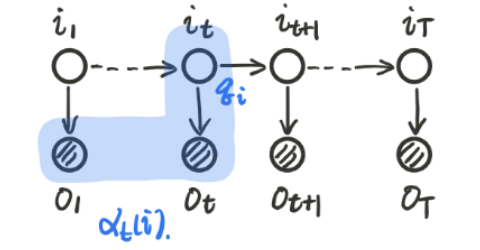
\includegraphics[scale=0.5]{figures/前向算法的拓扑结构.png}
    \caption{前向传播算法的拓扑结构}
\end{figure}

前向算法的主要思想是,在之前所有的观测变量$O_t$的前提下求出当前时刻的隐变量的概率,即
\begin{equation}
    P(O|\lambda)=\sum_{i=1}^{n} P(O,I_T=q_i|\lambda)=\sum_{i=1}^{n} \alpha_T(i)
\end{equation}

我们希望的是从$\alpha_1(i)$开始,一步一步向前推从而获得$\alpha_T$,也就是我们需要的是$\alpha_t(i)$和$\alpha_{t+1}(i)$具有某种递推关系,
下面我们来推导这种关系

\begin{mdframed}
    \begin{proposition}
        $\alpha_{t+1}(j)=b_j(O_{t+1})\cdot a_{ij}\cdot\alpha_i(i)$,其中$b_j(O_{t+1})=\sum_{k=1}^{M}\nu_k$
    \end{proposition}
\end{mdframed}

\begin{mdframed}[linewidth=0pt,backgroundcolor=gray!10]

    \begin{equation}
        \begin{aligned}
            \alpha_{t+1}(j)&=P(O_1,\cdots,O_t,O_{t+1},I_{t+1}=q_j|\lambda)\\
            &=\sum\limits_{i=1}^{N}P(O_1,\cdots,O_t,O_{t+1},I_{t}=q_i,I_{t+1}=q_j|\lambda)\\
            &=\sum\limits_{i=1}^{N}\underbrace{P(O_{t+1}|I_{t+1}=q_j,\lambda)}_{A}\underbrace{P(O_{1},O_{2},\cdots,O_{t},I_t=q_i,I_{t+1}=q_j|\lambda)}_{B}
        \end{aligned}
    \end{equation}

    其中$A$式刚好是观测概率矩阵的元素$b_j(O_{t+1})$

    \begin{equation}
        A=P(O_{t+1}|I_{t+1}=q_j,\lambda)=\sum_{k=1}^{M}b(O_{t+1}=\nu_k|I_{t+1=q_j},\lambda)=b_j(O_{t+1})
    \end{equation}

    主要来关注$B$,我们发现$B$还有关于$t+1$的项,我们想要这一项只和$t$及其之前的序列相关,因此对$B$做继续展开
    \begin{equation}
        \begin{aligned}
            B&=P(O_{1},O_{2},\cdots,O_{t},I_t=q_i,I_{t+1}=q_j|\lambda)\\
            &=P(I_{t+1}=q_j|O_{1},O_{2},\cdots,O_{t},I_t=q_i,\lambda)\cdot P(O_{1},O_{2},\cdots,O_{t},I_t=q_i|\lambda)\\
        \end{aligned}
    \end{equation}

    根据齐次马尔可夫假设
    \begin{equation}
        B=P(I_{t+1}=q_j|I_t=q_i,\lambda)\cdot P(O_{1},O_{2},\cdots,O_{t},I_t=q_i|\lambda)\\
    \end{equation}

    上式子左边第一项刚好是转移矩阵,第二项刚好是$\alpha_t(i)$所以
    \begin{equation}
        B=a_{ij}\cdot \alpha_t(i)
    \end{equation}

    然后我们把$A$和$B$最后的计算结果带回$\alpha_{t+1}(j)$
        \begin{equation}
            \alpha_{t+1}(j)=b_j(O_{t+1})\cdot a_{ij}\cdot \alpha_t(i)
        \end{equation}

\end{mdframed}

这个递推关系有什么意义呢?我们的联合概率分布是
\begin{equation}
    P(O|\lambda)=\sum_{i=1}^{n} P(O,I_T=q_i|\lambda)=\sum_{i=1}^{n} \alpha_T(i)
\end{equation}

利用递推关系,我们可以从简单的$\alpha_1$开始,用$\alpha_1$推导$\alpha_2$、$\alpha_2$推导$\alpha_3\cdots$,以此类推,最终算出来$\alpha_T(j)$,代入求和式就是联合概率分布。
而$\alpha_1$是只和一个状态结点和一个观测结点相关,因此是容易确定的。
\begin{figure}[H]
    \centering
    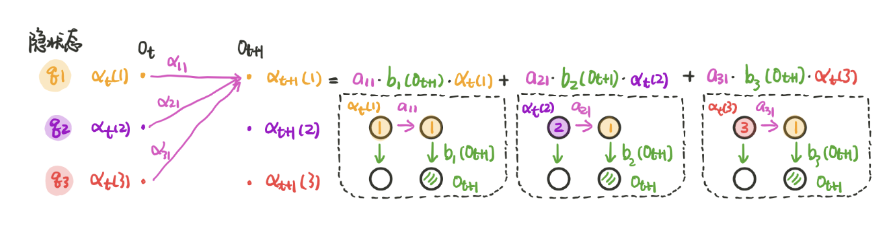
\includegraphics[scale=0.5]{figures/HMM前向传播示意图.png}
    \caption{HMM前向传播示意图}
\end{figure}

前向算法实际上是基于“状态序列的路径结构”递推计算联合概率分布的算法。其关键在于\textsl{局部计算前向概率,利用路径结构将前向概率递推到全局,从而减少每一次计算直接引用前一个时刻的计算结果,避免重复计算},
每次计算,隐状态的状态空间数为$N$,序列长度为$T$,因此这样利用前向计算算法的计算量是$O(N^2T)$阶的。


\section{后向算法}

后向概率的推导实际上比前向概率的理解要难一些,前向算法实际上是一个联合概率,而后向算法则是一个条件概率,所以后向的概率实际上比前向难求很多。

\begin{figure}[H]
    \centering
    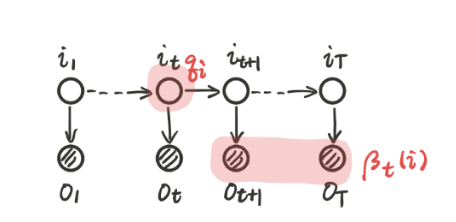
\includegraphics[scale=0.5]{figures/后向算法示意图2.png}
    \caption{后向算法示意图}
\end{figure}

我们设$\beta_{t}(i)=P(O_{t+1},\cdots,O_{T}|I_t=q_i,\lambda)$,计算观测的联合概率分布
\begin{equation}
    \begin{aligned}
        P(O|\lambda)&=P(O_1,O_2,\cdots,O_N|\lambda)\\
        &=\sum_{i=1}^{N}P(O_1,O_2,\cdots,O_N,I_1=q_i|\lambda)\\
        &=\sum_{i=1}^{N}P(O_1,O_2,\cdots,O_N|I_1=q_i,\lambda)\cdot P(I_1=q_i|\lambda)\\
        &=\sum_{i=1}^{N}P(O_1|O_2,\cdots,O_N,I_1=q_i|\lambda)\cdot P(O_2,\cdots,O_N,I_1=q_i|\lambda)\cdot\pi_i\\
        &=\sum_{i=1}^{N}P(O_1|I_1=q_i,\lambda)\cdot \beta_i(i)\cdot \pi_i\\
        &=\sum_{i=1}^{N}b_i(O_1)\cdot \beta_1(i)\cdot \pi_i
    \end{aligned}
\end{equation}

现在我们成功找到了$P(O|\lambda)$和第一个状态之间的关系,如下图所示
\begin{figure}[H]
    \centering
    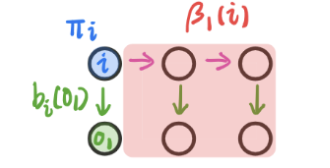
\includegraphics[scale=0.5]{figures/与第一个状态的关系.png}
    \caption{$P(O|\lambda)$与第一个状态的关系}
\end{figure}

现在我们要通过递推找最后一个状态和第一个状态的关系
\begin{equation}
    \begin{aligned}
        \beta_t(i)&=P(O_{t+1},\cdots,O_{T}|I_t=q_i)\\
        &=\sum_{j=1}^{N}P(O_{t+1},\cdots,O_{T}|I_t=q_i,i_{t+1}=q_j)\cdot P(I_{t+1}=q_j|I_t=q_i)
    \end{aligned}
\end{equation}

根据概率图模型,$I_t$和$t+1$后面所有的状态都没有关系,因此
\begin{equation}
    \begin{aligned}
        \beta_t(i)&=\sum_{j=1}^{N}P(O_{t+1},\cdots,O_T|I_{t+1}=q_j)\cdot a_{ij}\\
        &=\sum_{j=1}^{N}P(O_{t+1}|O_{t+1},\cdots,O_T,I_{t+1}=q_j)\cdot \underbrace{P(O_{t+2},\cdots,O_T|I_{t+1}=q_j)}_{\beta_{t+1}(j)}\cdot a_{ij}\\
        &=\sum_{j=1}^{N} b_j(O_{t+1})\cdot \beta_{t+1}(j)\cdot a_{ij}
     \end{aligned}
\end{equation}

马尔可夫链中每一个状态都是后一个状态的充分统计量,与之前的状态没有关系
\begin{equation}
    P(O_{t+1},\cdots,O_T|I_{t+1}=q_j,I_t=q_i)=P(O_{t+1},\cdots,O_T|I_{t+1}=q_j)
\end{equation}

通过这样的迭代方法从后往前推就可以得到$\beta_1(i)$的概率了,从而推断$P(O|\lambda)$。

\begin{figure}[H]
    \centering
    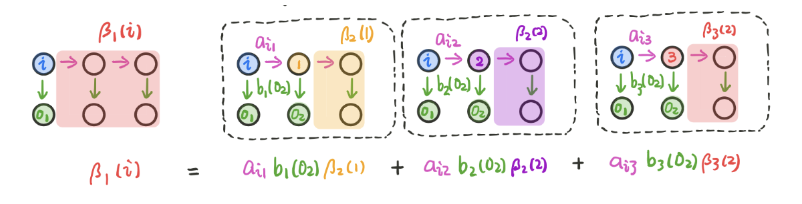
\includegraphics[scale=0.5]{figures/后向算法示意图.png}
    \caption{后向传播算法的拓扑结构}
\end{figure}
   \chapter{\textsl{Lagrange}力学}

\section{广义坐标}

\section{最小作用量原理}

使得泛函最小
\begin{equation}
    S[\mathcal{L}(q,\dot{q},t)]=\int_{t_1}^{t_2} \mathcal{L}(q(t),\dot{q}(t),t) dt
\end{equation}

\section{\textsl{Lagrange}方程}

由泛函的一阶变分并根据泛函极值条件可得拉格朗日方程
\begin{equation}
    \frac{\partial\ \mathcal{L}}{\partial q}-\frac{d}{dt}(\frac{\partial\ \mathcal{L}}{\partial \dot{q}})=0
\end{equation}

\section{对称量与守恒量}

在物理学中有三个基本的守恒量

\begin{enumerate}[itemindent=2em]
    \item 时间平移对称性$\ \Rightarrow\ $能量守恒;
    \item 空间平移对称性$\ \Rightarrow\ $动量守恒;
    \item 空间旋转对称性$\ \Rightarrow\ $角动量守恒;
\end{enumerate}

诺特定理给守恒量的存在提供了理论基础。

\begin{framed}
    \begin{theorem}
        (\textbf{诺特定理}) 如果系统的拉格朗日量在连续的连续无穷小变换$q\rightarrow q'=q'(\epsilon)$($\epsilon$是一阶小量)下保持不变,
        \begin{equation}
            \mathcal{L}(q(\epsilon),\dot{q}'(\epsilon),t)-\mathcal{L}(q,\dot{q},t)=0\ \Leftrightarrow\ \left.\frac{\partial \mathcal{L}(q(\epsilon),\dot{q}'(\epsilon))}{\partial \epsilon}\right|_{\epsilon=0}=0
        \end{equation}
        则系统必存在守恒量
        \begin{equation}
            \varLambda=\frac{\partial \mathcal{L}}{\partial \dot{q}}\left.\frac{d q'}{d \epsilon}\right|_{\epsilon=0}
        \end{equation}
    \end{theorem}
\end{framed}

\footnote{如果一个系统的拉格朗日量对于某个广义坐标$q_i$不显含(即对称性存在),那么对应的广义动量$p_i$是守恒的。}
\begin{mdframed}[backgroundcolor=gray!20,hidealllines=true]
    \textbf{proof}. 根据在连续无穷小变换下保持不变
    \begin{equation}
        \begin{aligned}
            \left.\frac{\partial \mathcal{L}(q(\epsilon),\dot{q}'(\epsilon))}{\partial \epsilon}\right|_{\epsilon=0}&=\left[\frac{\partial\mathcal{L}}{\partial q'}\frac{\partial q'}{\partial \epsilon}+\frac{\partial\mathcal{L}}{\partial \dot{q}'}\frac{\partial \dot{q}'}{\partial \epsilon}\right]_{\epsilon=0}=0
        \end{aligned}
     \end{equation}

     由欧拉-拉格朗日方程得到
     \begin{equation}
        \frac{d}{dt}(\frac{\partial\mathcal{L}}{\partial \dot{q}'})\cdot\frac{d q'}{d\epsilon}+\frac{\partial \mathcal{L}}{\partial \dot{q}'}\cdot \frac{d \dot{q}}{d\epsilon}=0
     \end{equation}

     因此
     \begin{equation}
        \frac{d}{dt}\left[\frac{\partial\mathcal{L}}{\partial \dot{q}'}\cdot \frac{dq'}{d\epsilon}\right]=0\ \Rightarrow\ \left.\frac{\partial\mathcal{L}}{\partial \dot{q}'}\cdot \frac{dq'}{d\epsilon}\right|_{\epsilon=0}=\varLambda
     \end{equation}

\end{mdframed}


这是诺特定理最简单的表述,他告诉我们如果一个作用量做没有外界给予的突变的情况下,一定存在一个守恒量。下面验证一下前面描述的三种变换下守恒量存在。

\subsection*{能量守恒}

首先在\textsl{时间均匀性},推出能量守恒定律,由于时间均匀,即时间平动下拉格朗日量形式保持不变,因此拉格朗日量不显含时间,因此
\begin{equation}
    \frac{d \mathcal{L}}{dt}=\frac{\partial \mathcal{L}}{\partial \dot{q}}\cdot \frac{\partial \dot{q}}{\partial t}+\frac{\partial \mathcal{L}}{\partial q}\cdot \frac{\partial q}{\partial t}
\end{equation}

根据\textsl{Euler-Lagrange方程},上面式子可以化为

\begin{equation}
    \frac{d}{dt}\left[\frac{\partial \mathcal{L}}{\partial \dot{q}}\cdot \frac{\partial q}{\partial t}\right]=\frac{d\mathcal{L}}{dt}
    \ \Rightarrow\ \frac{d}{d}\left[\frac{\partial \mathcal{L}}{\partial \dot{q}}\cdot \frac{\partial q}{\partial t}-\mathcal{L}\right]=0
\end{equation}

最终得到
\begin{equation}
    \varLambda=\dot{q}\cdot\frac{\partial\mathcal{L}}{\partial\dot{q}}-\mathcal{L}
    \label{eq3.10}
\end{equation}

封闭系统的拉格朗日量一般可以表述为
\begin{equation}
    \mathcal{L}=\frac{1}{2}m\dot{q}^2-U(q)
\end{equation}

代入(\ref{eq3.10}),得到
\begin{equation}
    m\dot{q}^2-\mathcal{L}=\frac{1}{2}m\dot{q}^2+U(q)=E
\end{equation}

这刚好是机械能守恒。


\subsection*{动量守恒}

\textsl{空间平移对称性}意味着拉格朗日量不显含有广义坐标$q$,由\textsl{Euler-Lagrange方程}有
\begin{equation}
    \frac{d}{dt}\left[\frac{\partial \mathcal{L}}{\partial \dot{q}}\right]=\frac{\partial \mathcal{L}}{\partial q}=0
\end{equation}

即
\begin{equation}
    \frac{\partial \mathcal{L}}{\partial \dot{q}}=p=Constant
\end{equation}

$p$我们常常称之为\textsl{广义动量}。例如势能场中的运动例子
\begin{equation}
    \mathcal{L}=\frac{1}{2}mv^2-U(r)
\end{equation}

广义坐标为位移$r$,则广义动量为
\begin{equation}
    p=\frac{\partial \mathcal{L}}{\partial v}=mv
\end{equation}

这刚好是线性动量一般的表达式。广义动量不仅能描述线性动量,也能描述角动量,考虑在二维平面势能场中运动的粒子,

\subsection*{角动量守恒}

角动量守恒描述的是\textsl{空间各向同性},注意到我们前面定义的变分是关于空间位移的变分$\delta r=r_1(t)-r_2(t)$,现在我们要换成旋转位移的变分$\delta \varphi=\varphi_1(t)-\varphi_2(t)$,根据最小作用量原理和泛函极值条件
\begin{equation}
    \delta \mathcal{L}=\frac{\partial \mathcal{L}}{\partial r}\delta r+\frac{\partial \mathcal{L}}{\partial \dot{r}}\delta \dot{r}=0
\end{equation}

我们把$\delta r$替换成和角度相关的量
\begin{equation}
    \begin{aligned}
        & \delta r=r\times \delta \varphi\\
        & \delta\dot{r} =\dot{r}\times \delta \varphi\\
    \end{aligned}
\end{equation}

再由拉格朗日方程
\begin{equation}
    \begin{aligned}
        & \frac{\partial \mathcal{L}}{\partial \dot{r}}=p\\
        & \frac{\partial \mathcal{L}}{\partial r}=\dot{p}\\
    \end{aligned}
\end{equation}

整理得到
\begin{equation}
    \delta \mathcal{L}=p\cdot(\dot{r}\times \delta\varphi)+\dot{p}\cdot(r\times \delta \varphi)=0
\end{equation}

注意这里$p,r,\varphi$都是矢量,那么根据矢量运算法则,可以把$\delta\varphi$提出得到
\begin{equation}
    \delta \varphi\cdot(r\times \dot{p}+\dot{r}\times p)=\delta \varphi\cdot\frac{d}{dt}\left[(r\times p)\right]=0
\end{equation}

由$\delta\varphi$的任意性,所以只能是对时间的导数项为$0$,即
\begin{equation}
    r\times p=\mathcal{M}=Constant
\end{equation}

这里向量$\mathcal{M}$称之为\textsl{角动量}。角动量守恒的条件为外力矩为零。


\section{条件极值}

如果泛函极值存在约束条件,往往是以下的形式
\begin{equation}
    f(q,\dot{q},t)=0
\end{equation}

由拉格朗日乘子法,构造新的泛函
\begin{equation}
    \mathcal{H}(q(t),\dot{q}(t),t)=\mathcal{L}(q(t),\dot{q}(t),t)+\lambda^T f(q,\dot{q},t)
\end{equation}

其中$\lambda(t)=(\lambda_1(t),\lambda_2(t),\cdots,\lambda_n(t))$,分别求导可得
\begin{equation}
    \left\{ 
        \begin{aligned}
        & \frac{\partial \mathcal{H}}{\partial q}-\frac{d}{dt}\cdot \frac{\partial \mathcal{H}}{\partial \dot{q}}=0\\
        & \frac{\partial \mathcal{H}}{\partial \lambda}-\frac{d}{dt}\cdot \frac{\partial \mathcal{H}}{\partial \dot{\lambda}}=f=0
    \end{aligned}
    \right.
\end{equation}


   
%% Prevent urls running into margins in bibliography
\setcounter{biburlnumpenalty}{7000}
\setcounter{biburllcpenalty}{7000}
\setcounter{biburlucpenalty}{7000}

%% Add bibliography
\printbibliography[heading=bibintoc,title=References]

%% ----------------------------------------------------------------------
%%    Appendix (Letters for chapters)
%% ----------------------------------------------------------------------

\appendix

\chapter{Source Code Example}
%\label{chapter:title}

\emph{Adding source code to your report/thesis is supported with the package {\normalfont\texttt{listings}}. An example can be found below. Files can be added using {\normalfont\texttt{\textbackslash lstinputlisting[language=<language>]\{<filename>\}}}.}

\begin{lstlisting}[language=Python]
"""
ISA Calculator: import the function, specify the height and it will return a
list in the following format: [Temperature,Density,Pressure,Speed of Sound].
Note that there is no check to see if the maximum altitude is reached.
"""

import math
g0 = 9.80665
R = 287.0
layer1 = [0, 288.15, 101325.0]
alt = [0,11000,20000,32000,47000,51000,71000,86000]
a = [-.0065,0,.0010,.0028,0,-.0028,-.0020]

def atmosphere(h):
    for i in range(0,len(alt)-1):
        if h >= alt[i]:
            layer0 = layer1[:]
            layer1[0] = min(h,alt[i+1])
            if a[i] != 0:
                layer1[1] = layer0[1] + a[i]*(layer1[0]-layer0[0])
                layer1[2] = layer0[2] * (layer1[1]/layer0[1])**(-g0/(a[i]*R))
            else:
                layer1[2] = layer0[2]*math.exp((-g0/(R*layer1[1]))*(layer1[0]-layer0[0]))
    return [layer1[1],layer1[2]/(R*layer1[1]),layer1[2],math.sqrt(1.4*R*layer1[1])]
\end{lstlisting}

\chapter{Task Division Example}
%\label{chapter:title}

\emph{If a task division is required, a simple template can be found below for convenience. Feel free to use, adapt or completely remove.}

\begin{table}[htb]
    \setlength\extrarowheight{4pt}
    \centering
    \caption{Distribution of the workload}
    \label{tab:taskdivision}
    \begin{tabularx}{\textwidth}{lXX}
        \toprule
        & Task & Student Name(s) \\
        \midrule
        & Summary & \\
        Chapter 1 & Introduction &  \\
        Chapter 2 &  & \\
        Chapter 3 &  & \\
        Chapter * &  & \\
        Chapter * & Conclusion &  \\
        \midrule
        & Editors & \\
        & CAD and Figures & \\
        & Document Design and Layout & \\
        \bottomrule
    \end{tabularx}
\end{table}

%\chapter{Cauchy-Schwarz不等式\\及其证明}

\section{定理描述}

\subsection*{一般形式}

Cauchy-Schwarz不等式的一般描述如下
\begin{theorem}
    已知$a_1,\cdots,a_n,b_1\cdots,b_n$是实数,则
    \begin{equation}
        (\sum\limits_{i=1}^{n}a_ib_i)^2\leqslant (\sum\limits_{i=1}^{n}a^2_i)(\sum\limits_{i=1}^{n}b^2_i) 
    \end{equation}

    等号成立的充分必要条件是
    \begin{equation}
        a_i=\lambda b_i,\ \ i=1,\cdots n
    \end{equation}
\end{theorem}

\subsection*{推广到复数形式}
不等式可以推广到复数。如何推广呢?不等式只有在实数时才有意义,对于复数则需要考虑角度和模长
大小关系。

\begin{theorem}
    已知$a_1,\cdots,a_n,b_1\cdots,b_n$是复数,则
    \begin{equation}
        |\sum\limits_{i=1}^{n}a_ib_i|^2\leqslant (\sum\limits_{i=1}^{n}|a_i|^2)(\sum\limits_{i=1}^{n}|b_i|^2) 
    \end{equation}

    等号成立的充分必要条件是
    \begin{equation}
        a_i=\lambda b_i,\ \ i=1,\cdots n
    \end{equation}
\end{theorem}

\subsection*{矩阵形式}

根据线性代数的理论:\textsl{任意正定对称矩阵都可以定义内积}。因此若$A=a_{ij}$为正定对称矩阵,则
$Cauchy$不等式存在
\begin{theorem}
    已知$(a_{ij})_{kl}$是正定对称矩阵,对于$x_1,\cdots,x_n,y_1.\cdots,y_n$是任意复数或者实数,则
    \begin{equation}
        |\sum\limits_{i=1}^{n}a_{ij}x_iy_j|\leqslant \sqrt{\sum\limits_{i,j=1}^{n}a_{ij}x_ix_j}
        \sqrt{\sum\limits_{i,j=1}^{n}a_{ij}y_iy_j}
    \end{equation}

    等号成立的充分必要条件是
    \begin{equation}
        a_i=\lambda b_i,\ \ i=1,\cdots n
    \end{equation}
\end{theorem}

\subsection*{无穷级数形式}

\begin{theorem}
    已知$a_1,\cdots,a_n,\cdots,b_1\cdots,b_n,\cdots$是复数,则
    \begin{equation}
        |\sum\limits_{i=1}^{\infty}a_ib_i|\leqslant 
        (\sum\limits_{i=1}^{\infty}|a_i|^2)^{\frac{1}{2}}
        (\sum\limits_{i=1}^{\infty}|b_i|^2)^{\frac{1}{2}}
    \end{equation}

    等号成立的充分必要条件是
    \begin{equation}
        a_i=\lambda b_i,\ \ i=1,\cdots ;\ \ \lambda\in \mathbb{C}
    \end{equation}
    \begin{equation}
        \sum\limits_{i=1}^{\infty}|a_i|^2<\infty
    \end{equation}
    \begin{equation}
        \sum\limits_{i=1}^{\infty}|b_i|^2<\infty
    \end{equation}
\end{theorem}

\subsection*{积分形式}

\begin{theorem}
    已知$f,g$是区间$[a,b]$上的连续函数,$f,g\in C[a,b]$,则
    \begin{equation}
        |\int_{a}^{b}f(x)g(x)dx|^2\leqslant \int_{a}^{b}|f(x)|^2dx \int_{a}^{b}|g(x)|^2dx 
    \end{equation}
\end{theorem}

\subsection*{$H\ddot{o}lder$不等式}
\begin{theorem}
    已知$a_1,\cdots,a_n,b_1\cdots,b_n$是复数,$p,q\geqslant 1$,$\frac{1}{p}+\frac{1}{q}=1$,则
    \begin{equation}
        |\sum\limits_{i=1}^{n}a_ib_i|\leqslant (\sum\limits_{i=1}^{n}|a_i|^p)^{\frac{1}{p}}
        (\sum\limits_{i=1}^{n}|b_i|^q)^{\frac{1}{q}} 
    \end{equation}
\end{theorem}

\subsection*{广义Cauchy-Schwarz不等式}

\begin{theorem}
    一般$n$维向量空间中的Cauchy-Schwarz不等式形式为
    \begin{equation}
        |a\cdot b|\leqslant \Vert a\Vert \Vert b\Vert
    \end{equation}
\end{theorem}

\section{余弦定律}
考虑三角形$\bigtriangleup ABC$,三条边的分量分别是
\begin{equation}
    \overrightarrow{a}=\overrightarrow{AB},\overrightarrow{b}=\overrightarrow{AC},
    \overrightarrow{c}=\overrightarrow{CB}=\vec{a}-\vec{b}
\end{equation}

\begin{figure}[H]
    \centering
    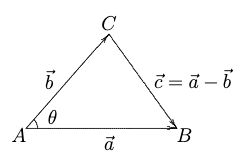
\includegraphics[scale=0.6]{figures/余弦定律.png}
    \caption{余弦定律}
\end{figure}

根据余弦定律$|\vec{a}|^2+|\vec{b}|^2-|\vec{a}-\vec{b}|^2=2|\vec{a}||\vec{b}|\cos{\theta}$以及余弦的性质$|\cos{\theta}|\leqslant 1$,可得
\begin{equation}
    |\vec{a}\cdot\vec{b}|\leqslant |\vec{a}||\vec{b}|
\end{equation}

这就是Cauchy-Schwarz不等式。他告诉我们Cauchy-Schwarz不等式的几何意义:三角形两边的内积小于两个向量长度的乘积。

\section{证明}

考虑$b$在$a$上的投影之差的最短距离,设
\begin{equation}
    \overrightarrow{c}=\vec{b}-\lambda \vec{a},\ \ \ \ \lambda\in \mathbb{R}
\end{equation}

$\vec{c}$的长度

\begin{eqnarray}
    |\vec{c}|^2=\vec{c}\cdot \vec{c}=|\vec{a}|^2\lambda^2+2\vec{a}\cdot \vec{b}\lambda +|b|^2>0
\end{eqnarray}

上式可视为$\lambda$的二次方程,且与$\lambda$轴没有交点

\begin{equation}
    \bigtriangleup = (2\vec{a}\vec{b})^2-4|\vec{a}|^2|\vec{b}|^2\leqslant 0
\end{equation}

因此有
\begin{equation}
    |\vec{a}\cdot \vec{b}|\leqslant |\vec{a}||\vec{b}|
\end{equation} % Create file to add

\end{document}
